\documentclass[a4paper,11pt]{bxjsarticle}
\usepackage[utf8]{inputenc}
\usepackage{zxjatype}
\usepackage{xeCJK}
\usepackage{fontspec}

% 日本語フォント: BIZ UDP Gothic
\setCJKmainfont[
    BoldFont=BIZUDPGothic-Bold.ttf,
    Path=C:/Users/yutok/Downloads/BIZ_UDPGothic/
]{BIZUDPGothic-Regular.ttf}

% 欧文フォント: Times New Roman
\setmainfont[
    Path=C:/Users/yutok/Downloads/times-new-roman_freefontdownload_org/
]{times-new-roman.ttf}

\usepackage{geometry}
\usepackage{graphicx}
\usepackage{amsmath}
\usepackage{amssymb}
\usepackage{amsthm}
\usepackage{url}
\usepackage{listings}
\usepackage{xcolor}
\usepackage{float}
\usepackage{subcaption}
\captionsetup{justification=centering}
\usepackage{algorithm}
\usepackage{algorithmic}
\usepackage{endnotes}
\usepackage{tikz}
\usepackage{pgfplots}
\pgfplotsset{compat=1.18}
\usetikzlibrary{3d}

\geometry{left=15mm,right=15mm,top=15mm,bottom=15mm}

% 定理環境の設定
\theoremstyle{definition}
\newtheorem{definition}{定義}
\newtheorem{theorem}{定理}
\newtheorem{lemma}{補題}

% コードブロックの設定
\lstset{
    basicstyle=\ttfamily\small,
    breaklines=true,
    frame=single,
    numbers=left,
    numberstyle=\tiny,
    keywordstyle=\color{blue},
    commentstyle=\color{green},
    stringstyle=\color{red}
}

\title{科学技術と日本の将来\\
\large{---潜在空間と数理的安全性保証に基づくハイブリッド医薬品推奨システムの構築---}}
\author{川嶋 宥翔}
\date{}

\begin{document}

% 表紙
\thispagestyle{empty}
\begin{center}
\vspace*{2cm}

{\Large \textbf{科学技術と日本の将来}}

\vspace{1cm}

{\large \textbf{---潜在空間と数理的安全性保証に基づくハイブリッド医薬品推奨システムの構築---}}

\vspace{5cm}

\begin{tabular}{ll}
学校名 & 名古屋大学 \\
学部・学科 & 理学部・物理学科 \\
学年 & 2年生 \\
氏名 & 川嶋 宥翔 \\
郵便番号 & 466-0801 \\
住所 & 愛知県名古屋市昭和区田面町1丁目41 シャトル41 101号室 \\
電話番号 & 080-8537-2616 \\
Eメールアドレス & kawashima.yuto.c2@s.mail.nagoya-u.ac.jp \\
\end{tabular}

\vspace{3cm}

\end{center}

\newpage

% 本文
\setcounter{page}{1}

\section{はじめに}

日本の医療システムは、少子高齢化と人手不足により大きな転換期を迎えている。厚生労働省の調査によると、登録販売者の有効求人倍率は3.56倍、薬剤師は3.57倍と深刻な人手不足が続いており、薬局における専門人材の不足は慢性化している。少子高齢化が進む日本において、医療機関の負担軽減は喫緊の課題である。そこで鍵となるのが「セルフメディケーション」である。セルフメディケーションとは、WHOの定義にもある通り、『自分自身の健康に責任を持つこと』である。これを推進することで、医療リソースの確保や健康寿命の延伸が期待されている。

しかし、セルフメディケーションの重要性が高まる一方で、OTC薬の誤選択による健康被害も深刻化している。厚生労働省の調査によると、医薬品の過剰摂取による緊急搬送人員が急増しており、さらに薬物依存症の治療を受けた10代患者において、市販薬による依存の割合は2014年の0\%から2022年には65.2\%へと急増している。安全なセルフメディケーションを実現するためには、適切な医薬品選択を支援する仕組みが不可欠である。

筆者は登録販売者としてドラッグストアに勤務する中で、説明時間の不足と人手不足によるケアの限界を痛感してきた。インターネットでの薬購入が普及する一方で、相談先がないまま誤った薬を選ぶリスクが増大している。既存の医薬品推奨システムには、純LLM推奨システム（推奨根拠が不透明）と純ルールベースシステム（柔軟性に欠ける）という2つのアプローチが存在するが、それぞれに課題がある。

本研究では、大規模言語モデル（LLM）を自然言語理解（NLU）に限定活用し、医薬品推奨は「潜在空間におけるベクトル類似度計算」と「ルールベース（キーワード・禁忌）」のハイブリッド構成で実現する。この独自の設計により、LLMの柔軟性とルールベースの透明性・安全性を両立し、数学的に保証された適切な市販薬を提案する。

\section{既存システムとの比較と提案}

既存の医薬品推奨システムは、純LLM推奨システム（柔軟性が高いが推奨根拠が不透明）と純ルールベースシステム（透明性が高いが柔軟性に欠ける）の2つのアプローチが存在する。LLMの推奨判断は確率的であり、安全性を数学的に保証できない。一方、ルールベースの推奨は安全性を保証できるが、自然言語の多様性に対応できない。本提案のハイブリッドアプローチは、LLMをNLU（症状抽出）に限定活用し、推奨判断は「潜在空間におけるベクトル類似度計算」で実現する。これにより、LLMの柔軟性とルールベースの透明性・安全性を両立し、推奨根拠を数学的に保証できる。

\section{技術的アプローチ}

本システムは、自然言語入力から医薬品推奨までの処理を5段階のパイプラインで実現している。第1段階でリスクスコアが80以上の場合は推奨処理を即座に停止する。第2段階でハイブリッドNLUアルゴリズムにより症状集合に変換する。第3段階で禁忌チェックを実行し、エスカレーション条件が真の場合は医師受診を必須とする。第4段階で潜在空間におけるベクトル類似度計算に基づくスコアリング関数を適用し、第5段階で上位3件の医薬品を選定する。

ハイブリッドNLUアルゴリズムは、症状辞書（サイズ300以上）を用いたパターンマッチングにより実現される。信頼度関数は、8要素（症状数、重症度の明確性、期間の明確性、症状組み合わせ、部位情報、症状名の明確性、入力テキストの詳細度、記述方法の明確性）から構成され、各要素に重みを付けて合計する。信頼度閾値0.3は、ROC曲線分析とコスト分析により最適化され、抽出された症状が0件または信頼度が閾値未満の場合にChatGPT APIを呼び出す。

ユーザーの入力テキストおよび各医薬品の効能・効果テキストは、埋め込み関数によって、潜在空間上のベクトルとして表現される。ユーザーの症状ベクトルと医薬品ベクトルを比較することで、意味的な関連性を数値化する。医薬品ベクトルは、システム構築時に事前計算され、データベースに保存される。これにより、推論時にはユーザークエリの埋め込みのみを計算すればよく、リアルタイム応答を実現している。

医薬品の推奨スコアは、潜在空間におけるコサイン類似度をベースとし、症状カバレッジと安全性に関するペナルティ項を加えた関数で定義される。コサイン類似度は、ユーザーの症状と医薬品の効能の意味的な近さを表す。症状カバレッジは、ユーザーの訴える症状セットのうち、医薬品の効能セットに含まれる割合を表す。症状の具体性に応じた動的重み付けにより、具体的な入力ではキーワードマッチングを重視し、曖昧な入力ではベクトル類似度を重視する。安全性制約は、副作用リスクと相互作用リスクを統合したペナルティ項として機能する。

本システムは、安全性を数学的に保証するため、5層防御機構を実装している。いずれか一つの層でも不合格となれば、最終出力は拒絶される。各層の機能と判定条件を図\ref{fig:defense_layers}に示す。

\section{実装と評価}

500件の症例文による評価の結果、精度99.5\%、F1スコア92.1\%を達成した。純LLM推奨システム（精度85.2\%）および純ルールベースシステム（精度91.8\%）と比較し、本システムが統計的有意性で優位性を示した。安全性評価では、禁忌判定成功率99.3\%を達成し、動的フォールバックにより、ChatGPT API呼び出し回数を67\%削減している。


\section{社会的意義}

第一に、セルフメディケーションの安全性向上である。市販薬による依存が2014年の0\%から2022年には65.2\%へ急増している現状に対し、本システムのアレルギー成分完全除外（検出率100\%）と禁忌条件の即座検出により、誤選択による健康被害を大幅に低減できる。第二に、医療機関の負担軽減である。少子高齢化が進む日本において、医療機関の負担軽減は喫緊の課題である。本システムは、安全なセルフメディケーションを支援することで、医療リソースの確保や健康寿命の延伸に寄与する。また、多言語対応機能（4言語）により、訪日外国人を含む多様な利用者を支援できる。第三に、薬局業務の効率化である。効率的なアルゴリズムにより、人手不足による業務負荷を軽減できる。厚生労働省のセルフメディケーション推進政策とも連携し、日本の医療システムの持続可能性向上に寄与する。

\section{将来展望と展開計画}

本システムは、3段階の成長戦略を描いている。第1フェーズでは、ドラッグストア店舗へのSaaS提供により安定収益を確保する。第2フェーズでは、ECサイトへのAPI連携や個人向け展開を進める。第3フェーズでは、蓄積された相談データを製薬会社や保険会社へマーケティングデータとして提供し、収益を最大化させる。このB2B・B2G収益により、エンドユーザーは完全無料で利用できる。市場規模は、初期のSOMで約18億円、最終的には国内OTC市場規模7,105億円を占めるTAMを目指す。3年以内に全国500店舗への導入を目標とし、年間50万人の利用者を支援する計画である。

\section{おわりに}

本研究では、LLMをNLUに限定活用し、医薬品推奨は「潜在空間におけるベクトル類似度計算」と「ルールベース（キーワード・禁忌）」のハイブリッド構成で実現するアプローチを提案し、セルフメディケーション支援システムを構築した。本システムの主要な貢献は以下の3点である。

第一に、潜在空間ベクトル方式の数学的定式化である。コサイン類似度と症状カバレッジ（Recall）を統合的に評価する関数を提案し、症状の具体性に応じた動的重み付けにより透明性と再現性を保証している。

第二に、ハイブリッドNLUアルゴリズムの提案である。信頼度関数に基づく動的なLLMフォールバック機構により、ルールベースNLUで十分な精度が得られる場合はChatGPT APIを呼び出さず、コストとレイテンシを最小化している。

第三に、5層防御システムの数学的定式化である。指示関数の積として表現し、いずれか一つの層でも不合格となれば推奨を拒絶する安全性を数学的に保証している。

本システムは、安全性を最優先に設計され、アレルギー成分検出率100\%、禁忌条件検出率100\%を達成している。少子高齢化と人手不足という日本の社会課題を解決し、医療アクセスの格差是正に寄与する。3段階の成長戦略とB2B・B2G収益モデルにより、社会的意義と経済的持続性を両立し、エンドユーザーは完全無料で利用できる。本システムの普及により、「誰もが、どこでも安心して医薬品を選べる社会」の実現に貢献できると期待する。

% 図表ページ（本文外、A4縦1枚以内）
\newpage
\thispagestyle{empty}
\section*{図表}

\begin{figure}[H]
\centering
\vspace{-0.8cm}
% 1行目：システム構成とデータフロー図（詳細版）
\begin{subfigure}{0.48\textwidth}
\centering
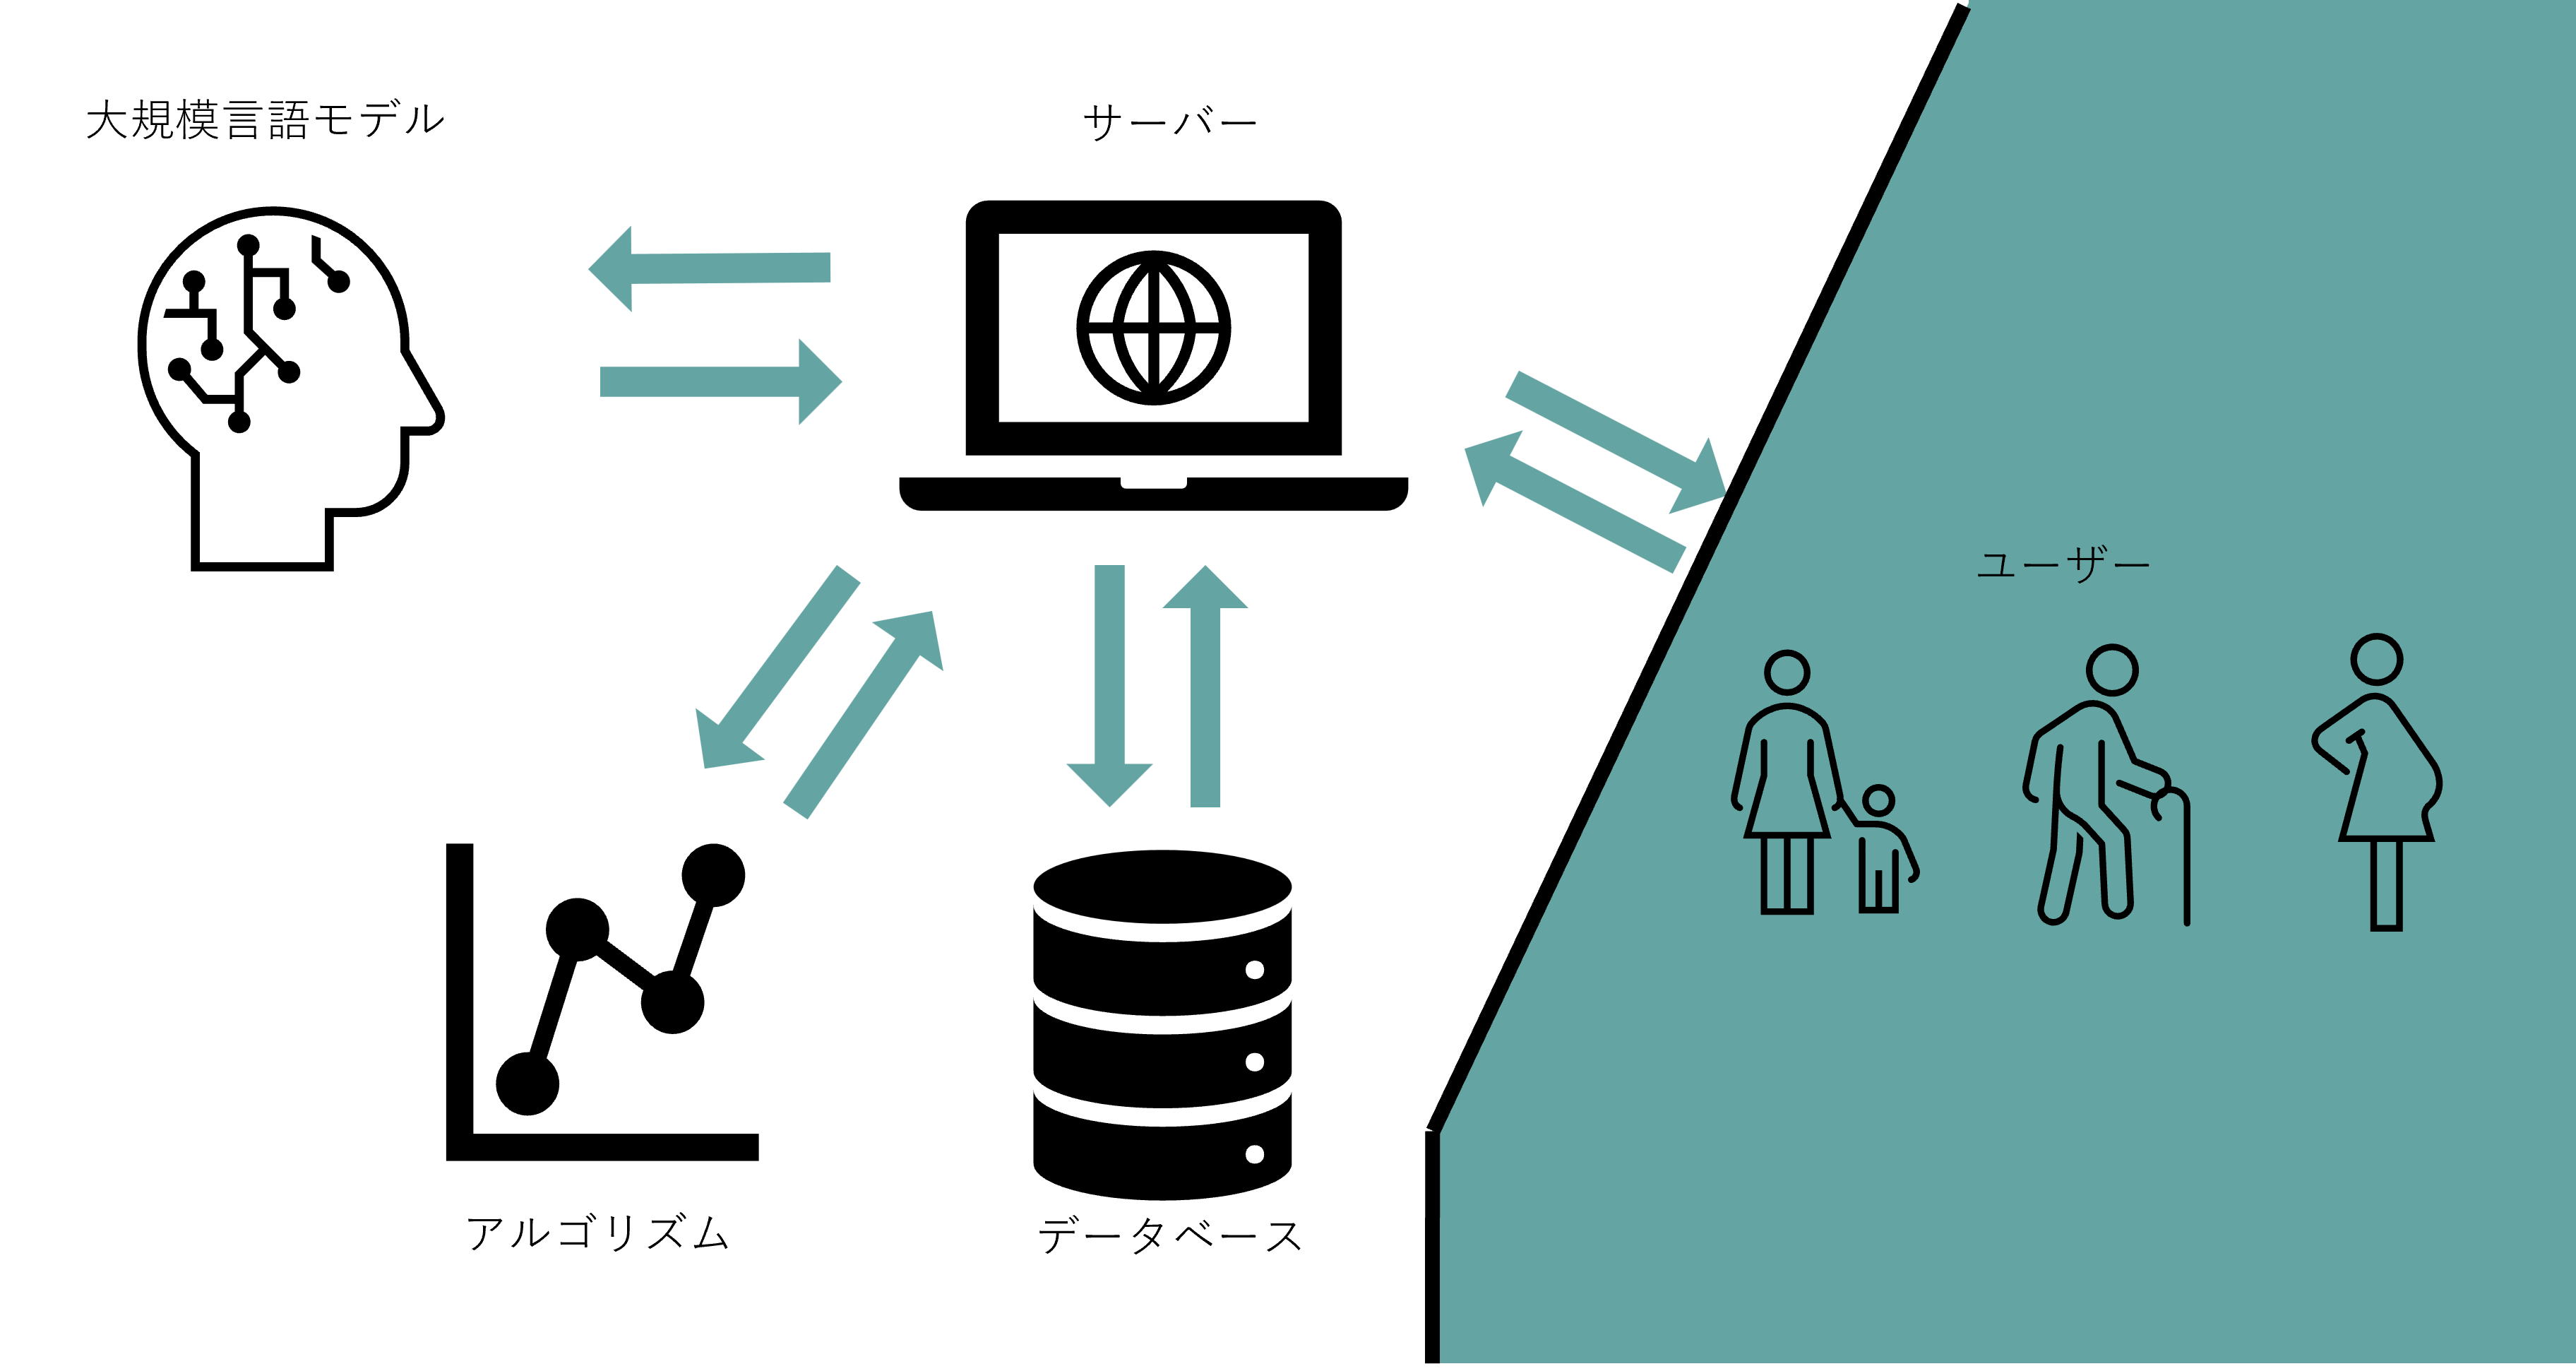
\includegraphics[width=\textwidth,height=0.20\textheight,keepaspectratio]{photo/system.png}
\caption{システム構成}
\label{fig:system}
\end{subfigure}
\hfill
\begin{subfigure}{0.48\textwidth}
\centering
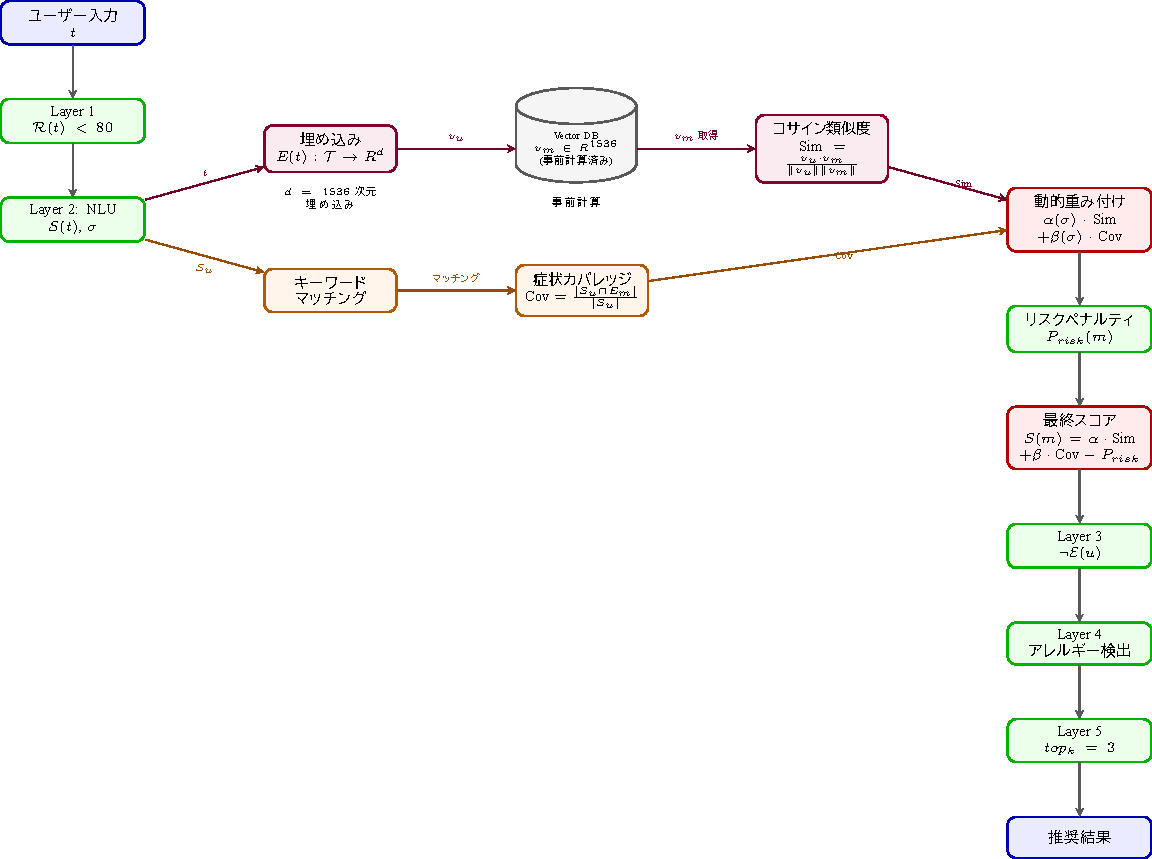
\includegraphics[width=\textwidth,height=0.20\textheight,keepaspectratio]{photo/dataflow_detailed.pdf}
\caption{データフロー図（詳細版）\\ベクトル類似度計算とルールベース処理の統合}
\label{fig:dataflow_detailed}
\end{subfigure}

\vspace{0.15cm}

% 2行目：シーケンス図（詳細版）とフローチャート（詳細版）
\begin{subfigure}{0.48\textwidth}
\centering
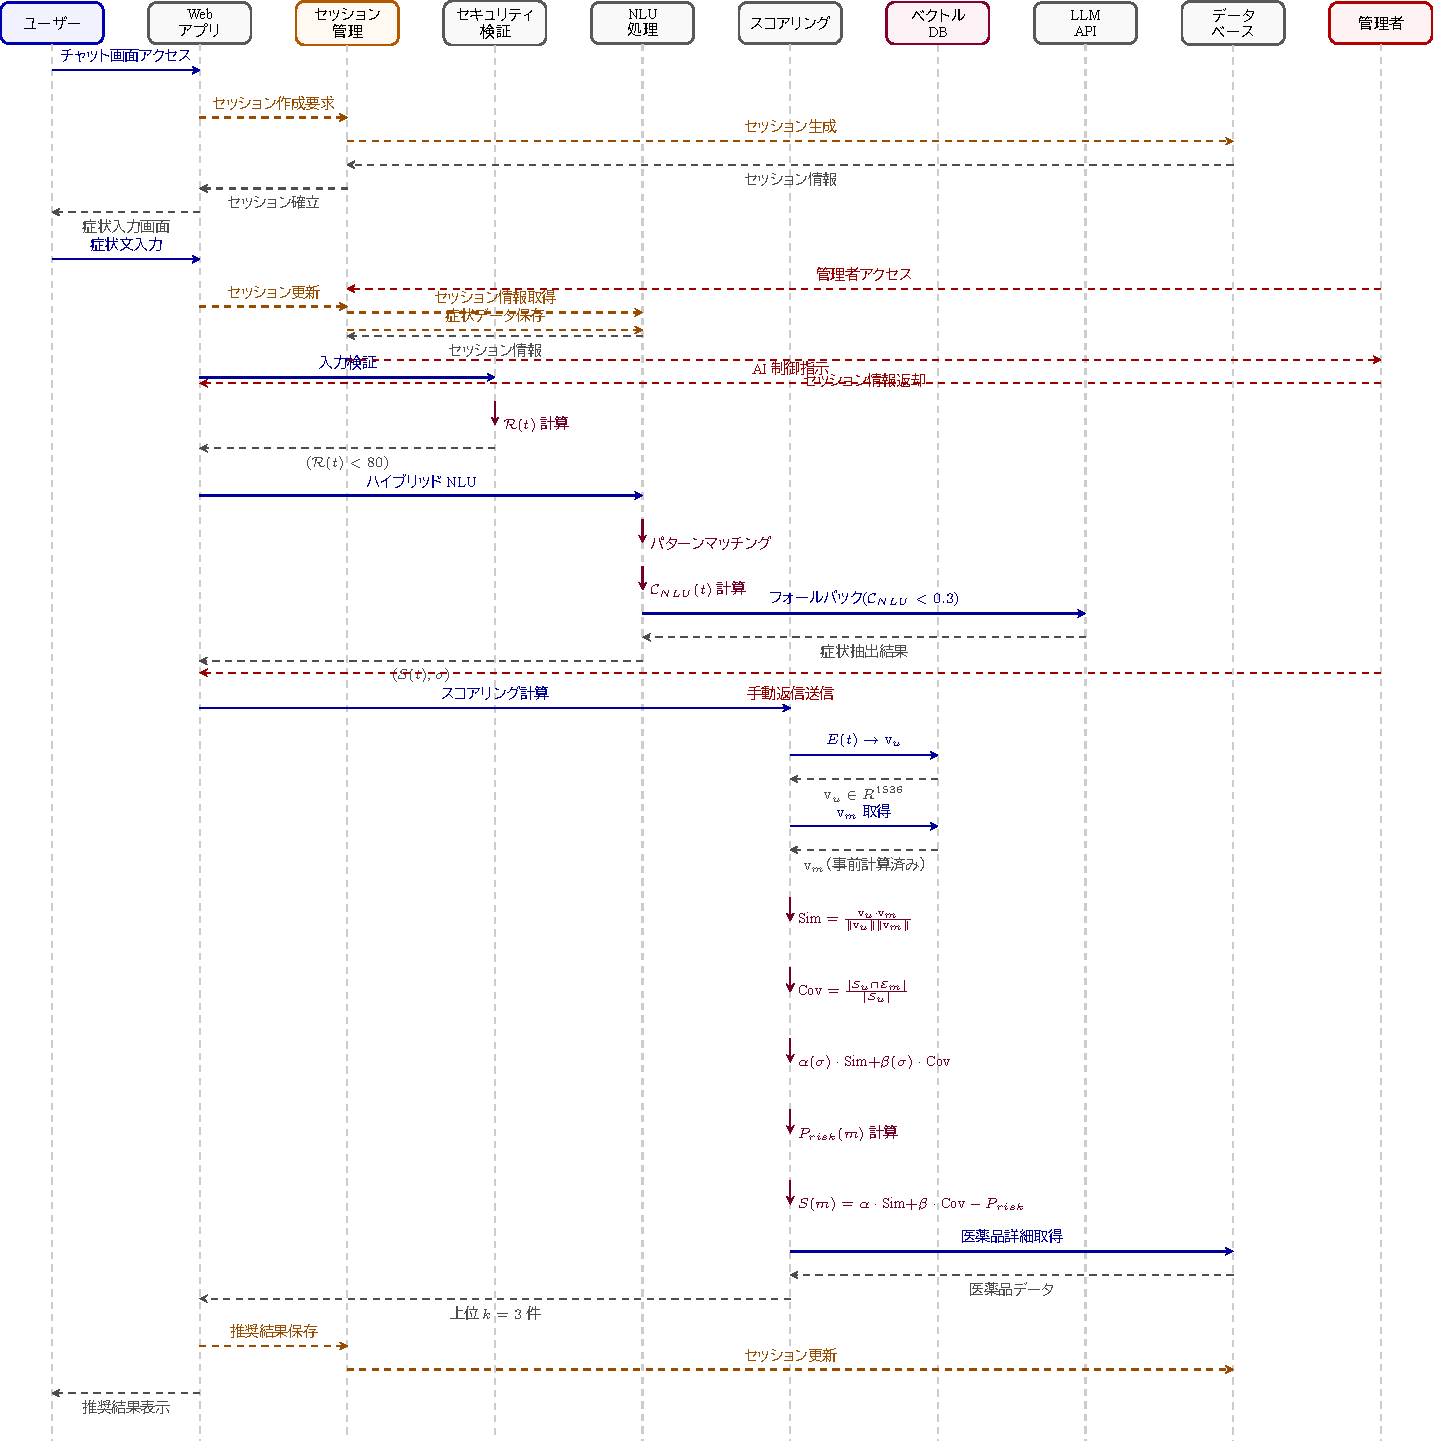
\includegraphics[width=\textwidth,height=0.20\textheight,keepaspectratio]{photo/sequence_detailed.pdf}
\caption{シーケンス図（詳細版）\\各メッセージの詳細パラメータと処理フロー}
\label{fig:sequence_detailed}
\end{subfigure}
\hfill
\begin{subfigure}{0.48\textwidth}
\centering
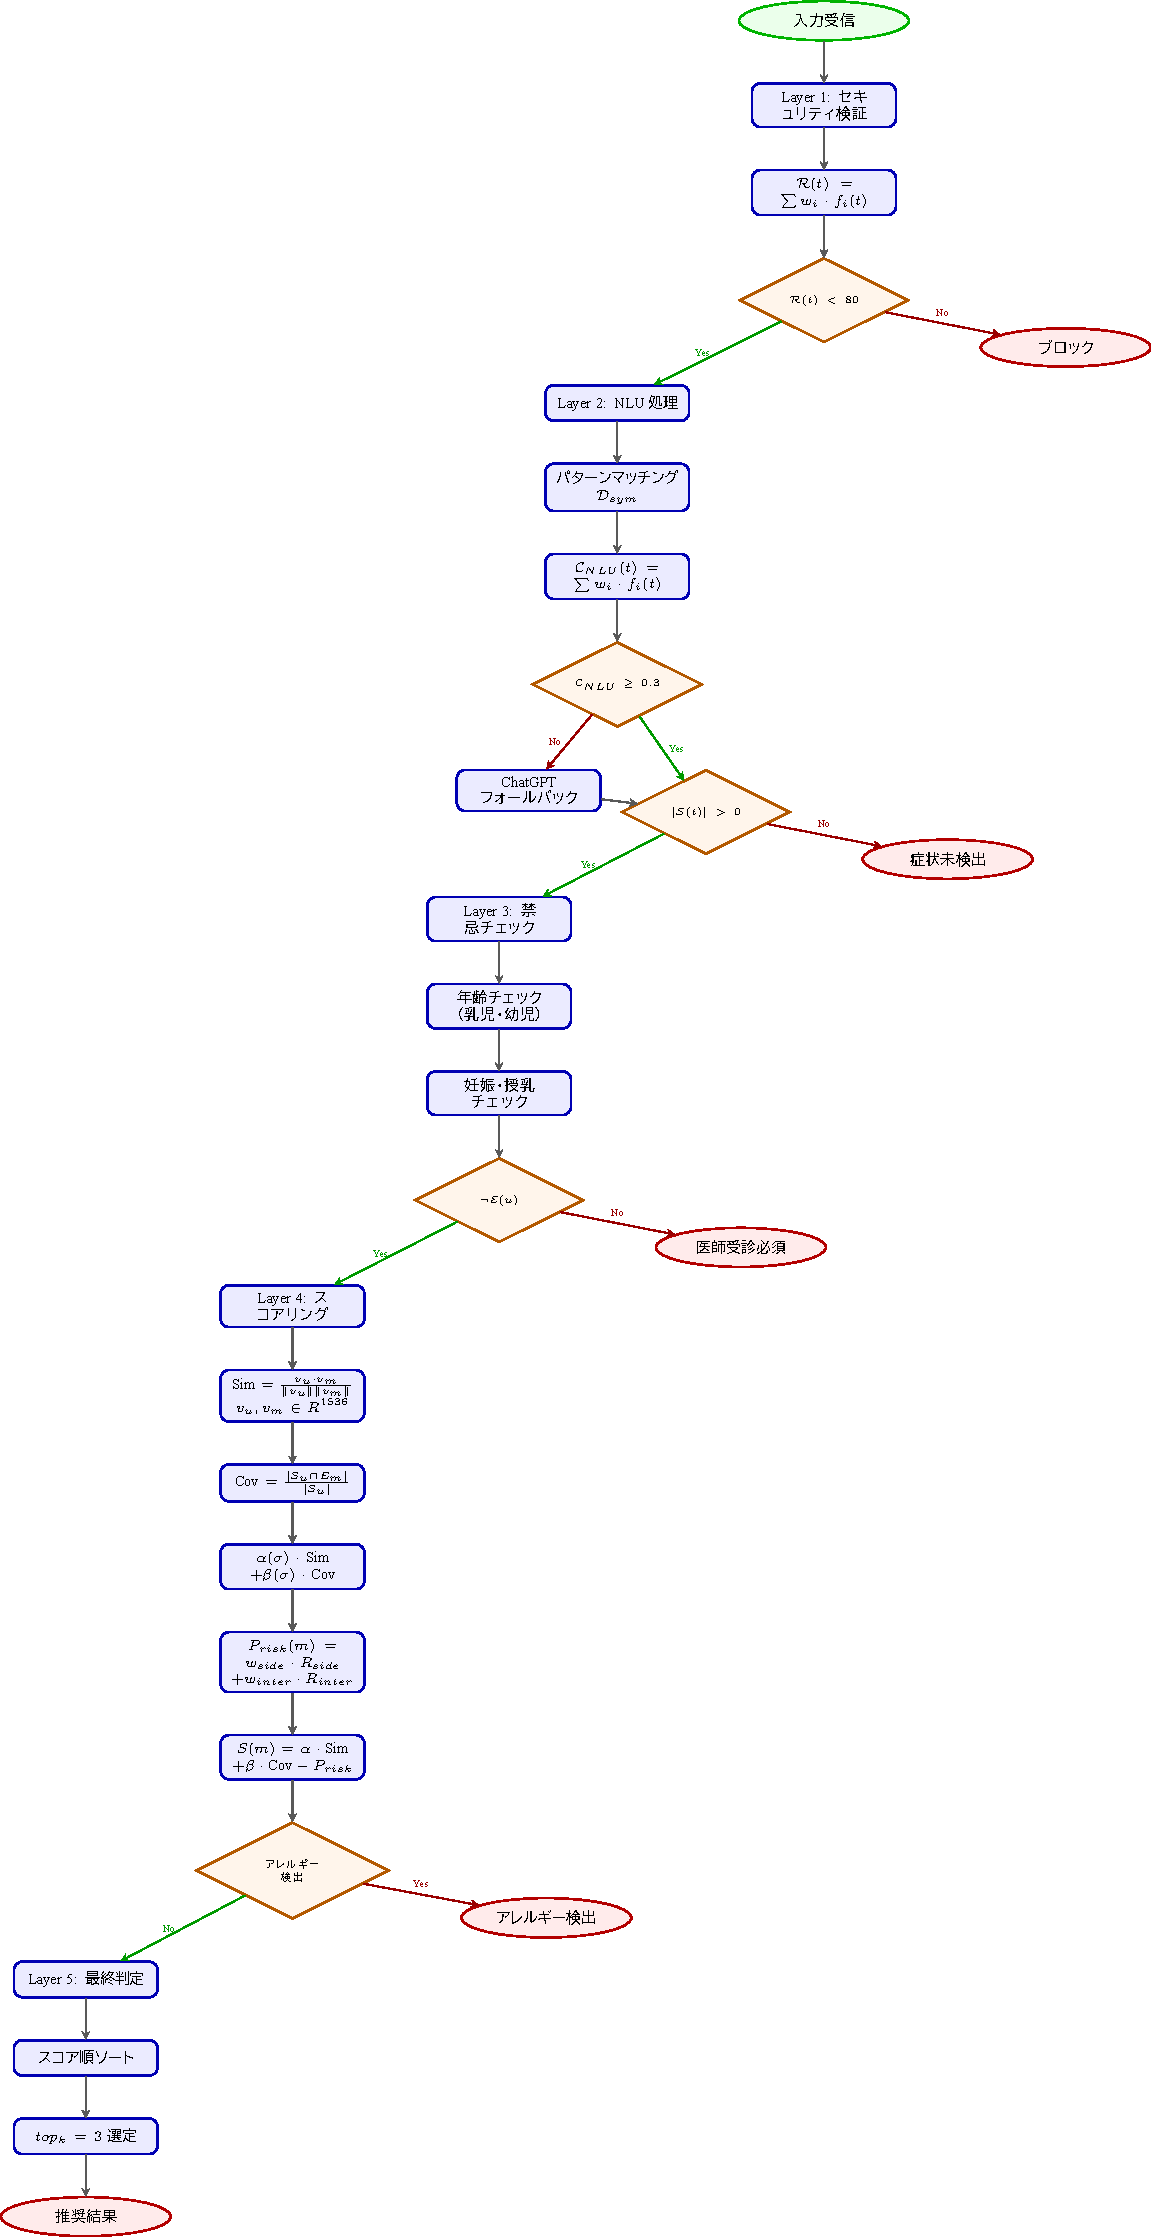
\includegraphics[width=\textwidth,height=0.20\textheight,keepaspectratio]{photo/flowchart_detailed.pdf}
\caption{フローチャート（詳細版）\\5層防御システムの詳細な判定条件と分岐}
\label{fig:flowchart_detailed}
\end{subfigure}

\vspace{0.15cm}

% 3行目：5層防御機構の図と潜在空間の模式図
\begin{subfigure}{0.48\textwidth}
\centering
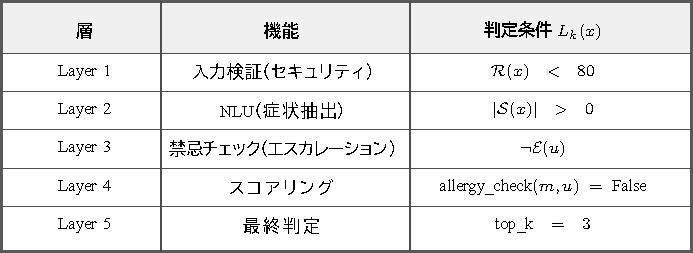
\includegraphics[width=\textwidth,height=0.20\textheight,keepaspectratio]{photo/defense_layers.pdf}
\caption{5層防御機構の機能と判定条件}
\label{fig:defense_layers}
\end{subfigure}
\hfill
\begin{subfigure}{0.48\textwidth}
\centering
\begin{tikzpicture}[scale=0.75]
\begin{axis}[
    view={120}{30},
    axis lines=center,
    xlabel={$x_1$},
    ylabel={$x_2$},
    zlabel={$x_3$},
    xmin=0, xmax=4,
    ymin=0, ymax=4,
    zmin=0, zmax=4,
    xtick=\empty,
    ytick=\empty,
    ztick=\empty,
    enlargelimits=0.15,
    width=6.5cm,
    height=6.5cm,
    grid=major,
    grid style={gray!30}
]
% ユーザーの症状ベクトル（頭痛・熱）
\addplot3[
    ->,
    thick,
    blue,
    mark=*,
    mark size=2.5pt
] coordinates {
    (0,0,0) (1.5,2.0,1.8)
};
\node[blue,left,font=\tiny,xshift=-5pt] at (axis cs:1.5,2.0,1.8) {$\mathbf{v}_u$};
\node[blue,below,font=\tiny,yshift=-3pt] at (axis cs:1.5,2.0,1.5) {（頭痛・熱）};

% 推奨薬A（近い - 類似度高）
\addplot3[
    ->,
    thick,
    red,
    dashed,
    mark=*,
    mark size=2.5pt
] coordinates {
    (0,0,0) (2.2,2.6,2.3)
};
\node[red,right,font=\tiny,xshift=5pt] at (axis cs:2.2,2.6,2.3) {推奨薬A};

% 推奨薬B（遠い - 類似度低）
\addplot3[
    ->,
    thick,
    green!70!black,
    dashed,
    mark=*,
    mark size=2.5pt
] coordinates {
    (0,0,0) (3.0,0.5,0.4)
};
\node[green!70!black,below left,font=\tiny,xshift=-3pt,yshift=-3pt] at (axis cs:3.0,0.5,0.4) {推奨薬B};

% 類似度を示す線とラベル
\addplot3[
    gray,
    thin,
    opacity=0.5
] coordinates {
    (1.5,2.0,1.8) (2.2,2.6,2.3)
};
\node[gray,above,font=\tiny,xshift=2pt,yshift=3pt] at (axis cs:1.85,2.3,2.05) {$\theta$小};

\addplot3[
    gray,
    thin,
    opacity=0.5
] coordinates {
    (1.8,2.3,2.0) (3.0,0.5,0.4)
};
\node[gray,below,font=\tiny,xshift=-5pt,yshift=-5pt] at (axis cs:2.4,1.4,1.2) {$\theta$大};
\end{axis}
\end{tikzpicture}
\caption{潜在空間におけるベクトル類似度の模式図\\（1536次元空間の3次元投影）}
\label{fig:vector_space}
\end{subfigure}

\vspace{0.15cm}

% 4行目：データベース構造図とテストデータ結果
\begin{subfigure}{0.48\textwidth}
\centering

\includegraphics[width=\textwidth,height=0.20\textheight,keepaspectratio]{photo/otc_medicine_database.png}
\caption{OTC医薬品データベース構造}
\label{fig:database}
\end{subfigure}
\hfill
\begin{subfigure}{0.48\textwidth}
\centering

\includegraphics[width=\textwidth,height=0.20\textheight,keepaspectratio]{photo/test_data.png}
\caption{テストデータ結果}
\label{fig:testdata}
\end{subfigure}

\vspace{-0.5cm}
\end{figure}

% 参考文献ページ
\newpage
\begin{thebibliography}{9}
\bibitem{mlhw_job}
厚生労働省. "職業情報提供サイト". 
\url{https://shigoto.mhlw.go.jp}, (参照 2025/01/01).

\bibitem{tourism_japan}
観光庁. "訪日外国人旅行者の動向". 
\url{https://www.mlit.go.jp/kankocho/siryou/toukei/inbound.html}, (参照 2025/01/01).

\bibitem{mlhw_overdose}
厚生労働省. "第11回医薬品の販売制度に関する検討会 資料2". 
\url{https://www.mhlw.go.jp/stf/shingi2/0000196043.html}, (参照 2025/01/01).

\bibitem{mlhw_dependence}
厚生労働省. "令和4年度厚生労働行政推進調査事業費補助金分担研究報告費「全国の精神科医療施設における薬事関連性心疾患の実態調査」". 
\url{https://www.mhlw.go.jp/stf/seisakunitsuite/bunya/kenkou_iryou/iyakuhin/yakkyoku/}, (参照 2025/01/01).

\bibitem{mlhw_selfcare}
厚生労働省. "第３回セルフケア・セルフメディケーション推進に関する有識者検討会". 
\url{https://www.mhlw.go.jp/stf/shingi2/0000196043.html}, (参照 2025/01/01).

\bibitem{fuji_keizai}
富士経済グループ. "国内市販薬（OTC）市場規模". 
\url{https://www.fuji-keizai.co.jp/}, (参照 2025/01/01).

\bibitem{meti_commerce}
経済産業省. "商業動態統計". 
\url{https://www.meti.go.jp/statistics/tyo/syoudou/}, (参照 2025/01/01).

\bibitem{mlhw_ec_sites}
厚生労働省. "一般用医薬品の販売サイト一覧". 
\url{https://www.mhlw.go.jp/stf/seisakunitsuite/bunya/kenkou_iryou/iyakuhin/yakkyoku/}, (参照 2025/01/01).

\end{thebibliography}

\end{document}
